\documentclass[11pt, notitlepage,  letterpaper]{article}


%% Horizontal Lengths - Max 6.5
\setlength{\footskip}{0.5in}
\setlength{\hoffset}{0in}
\setlength{\oddsidemargin}{-.2in}
\setlength{\evensidemargin}{-.2in}
%\setlength{\textwidth}{6.9in}
\setlength{\textwidth}{6.6in}

%% Vertical Lengths - Max 9.0
\setlength{\headheight}{0in} \setlength{\topskip}{0in}
\setlength{\voffset}{0in} \setlength{\topmargin}{0.5in}
\setlength{\textheight}{8.4in}

%\usepackage{fancyheadings}

\usepackage{url}
\usepackage[]{epsfig,amsmath}[]


%\pagestyle{headings}
%\pagestyle{fancy}
\pagenumbering{arabic}


%%%%%%%%%%%%%%%%%%%%%%%%%%%%%%%%%%%%%%%%%%%%%%%%%%%%%%%%%%%%%%%%%%%%%%
% New definitions and commands
\newtheorem{define}{Definition}[section]
\newtheorem{theorem}[define]{Theorem}
\newtheorem{question}[define]{Question}
\newtheorem{problem}[define]{Problem}


%**************************************


\begin{document}
%\title{
%{Solving Two-dimensional Forward Problems on an Annulus}\\{Using
%Spectral Fourier Methods}}
%
%\vfill
%\author{S.\ Choe \\ skchoe@cs.utah.edu \and R.\ M.\ Kirby \\ kirby@cs.utah.edu}
%
%\renewcommand{\today}{Jan 30th, 2004}
%
%\maketitle

%\begin{abstract}
%In this report, we present a spectral Fourier method for solving a
%Poisson equation with Dirichlet and Neumann boundary conditions
%respectively on an annulus domain. By using the tensor product
%between spectral and Fourier bases, we could apply the high-order
%method on the annulus domain. The fast Fourier transform allowed
%the rapid convergence on the radius to be maintained to all
%angular direction on the annulus.
%\end{abstract}

%\noinden {\bf Keywords: Spectral Element Methods, Poisson Equation}

%\tableofcontents

%-------------------------------------------------------------------------------
\clearpage

\section{Formulation of Boundary Element Method on a Circle}
In this section, we define a differential equation which satisfies
Laplace equation defined on a circle $\gamma$ as follows:
\begin{itemize}
\item {\bf Domain} : A Disk of radius 1.
\item {\bf Boundary Condition} : {\bf Outer} normal vectors.
\item {\bf Analytic solution} : $u(x,y) = x^2 - y^2$.
\item {\bf Orientation of Integral} : Counter clock wise.
\end{itemize}

Note that, regardless of direction of normal vectors,
mathematically this formulation should gives an unique numerical
solution.

According to boundary element method, we can set up the following
relation:

\begin{eqnarray}
\frac{1}{2}u(x) = -\int_{\gamma} u(z) \nabla G(z,x)\cdot {\bf n}
dz + \int_{\gamma} \frac{\partial u}{\partial n}(z) G(z, x) dz.
\end{eqnarray}

By discretization with element $E_j$ on $\gamma$, $j=1 \dots N$,

\begin{eqnarray}
\frac{1}{2}u(x) =  &-&\sum_{j=1}^{N}\int_{E_j} u(z) \nabla
G(z,x)\cdot {\bf n} dz + \sum_{j=1}^{N}\int_{E_j} \frac{\partial
u}{\partial n}(z) G(z, x) dz.
\end{eqnarray}


Let ${x_1, \dots, x_N}$ be the center points of elements ${E_1,
\dots, E_N}$. The we can approximate above equation by

\begin{eqnarray}
\frac{1}{2}u(x_i) = - \sum_{j=1}^{N}u(x_j)\int_{E_j} \nabla
G(z,x_i)\cdot {\bf n} dz + \sum_{j=1}^{N}\frac{\partial
u}{\partial n}(x_j)\int_{E_j} G(z, x_i) dz.
\end{eqnarray}


Define
\begin{eqnarray}
\alpha_j^i &=& \int_{E_j}G(z,x_i)dz\\
\beta_j^i &=& \int_{E_j}\nabla G(z,x_i)\cdot {\bf n} dz.
\end{eqnarray}
Then we can rearrange above equation by putting unknowns to left
and known values to right side as follows:

\begin{eqnarray}
\frac{1}{2} u(x_i) &+& \sum_{j=1}^N \beta_j^iu(x_j) = \sum_{j=1}^N
\alpha^i_j\frac{\partial u}{\partial n}(x_j),
\end{eqnarray}
for all $i,j = 1 \dots N$.

This enables to set up the following system of linear equations
for $u(x_j), j = 0, \dot, N$.

\begin{eqnarray}
\label{mat1}
\begin{bmatrix}
    \frac{1}{2}+\beta^1_1& \beta^1_2& \cdots & \beta^1_N \\
    \beta^2_1& \frac{1}{2}+\beta^2_2& \cdots & \beta^2_N\\
    \vdots& \vdots& \ddots& \vdots\\
    \beta^N_1& \beta^N_2& \cdots & \frac{1}{2} + \beta^N_N \\
\end{bmatrix}
\begin{bmatrix}
    u(x_1)    \\
    u(x_2)    \\
    \vdots      \\
    u(x_N)    \\
\end{bmatrix}
=
\begin{bmatrix}
    \sum_{j=1}^N \alpha^1_j\frac{\partial u}{\partial n}(x_j)   \\
    \sum_{j=1}^N \alpha^2_j\frac{\partial u}{\partial n}(x_j)   \\
    \vdots  \\
    \sum_{j=1}^N \alpha^N_j\frac{\partial u}{\partial n}(x_j)   \\
\end{bmatrix}.
\end{eqnarray}

Note that $\{\alpha^i_j, \beta^i_j\}$ in  (\ref{mat1}) assume the
condition defined in the beginning(CCW, Outer normal).

Mathematically, the original problem has same result as the case
when we have both clockwise orientation and inward normal vector.
In boundary element formulation, this fact can be seen through the
change in (\ref{mat1}), since $\{\alpha^i_j, \frac{\partial
u}{\partial n}(x_j)\}$ have opposite signs but $\{\beta^i_j\}$ has
no sign change.

\begin{itemize}
\item Radius 1cm
\item Number of elements: $2^6 \cdots 2^{12}$
\item Slope: 1.45xx
\end{itemize}

\begin{figure}[h]
    \begin{center}
    \epsfig{file = circle_htest_6_12.eps, width = 12cm}
    \caption{This figure is showing the h-convergence test for above problem}
    \end{center}
\end{figure}


\section{Case: Clockwise Orientation with Outer normal}
In this section we define shortly a slightly different example
based on the initial definition of example at previous section.

\begin{itemize}
\item {\bf Domain} : A Disk of radius 1.
\item {\bf Boundary Condition} : {\bf Outer} normal vectors.
\item {\bf Analytic solution} : $u(x,y) = x^2 - y^2$.
\item {\bf Orientation of Integral} : Clock wise.
\end{itemize}

This cause the changes to each element of formulation above:
\begin{itemize}
\item {\bf $\alpha^i_j$} : Sign Change
\item {\bf $\beta^i_j$} : Sign Change
\item {\bf $\frac{\partial u}{\partial n}(x_j)$} : No Change.
\end{itemize}

With the same meaning of notation as (\ref{mat1}), we can set up
the system of linear equation for this problem by modifying signs:


\begin{eqnarray}
\label{mat2}
\begin{bmatrix}
    \frac{1}{2}-\beta^1_1& -\beta^1_2& \cdots & -\beta^1_N \\
    -\beta^2_1& \frac{1}{2}-\beta^2_2& \cdots & -\beta^2_N\\
    \vdots& \vdots& \ddots& \vdots\\
    -\beta^N_1& -\beta^N_2& \cdots & \frac{1}{2} - \beta^N_N \\
\end{bmatrix}
\begin{bmatrix}
    u(x_1)    \\
    u(x_2)    \\
    \vdots      \\
    u(x_N)    \\
\end{bmatrix}
=
\begin{bmatrix}
    - \sum_{j=1}^N \alpha^1_j\frac{\partial u}{\partial n}(x_j)   \\
    - \sum_{j=1}^N \alpha^2_j\frac{\partial u}{\partial n}(x_j)   \\
    \vdots  \\
    - \sum_{j=1}^N \alpha^N_j\frac{\partial u}{\partial n}(x_j)   \\
\end{bmatrix}.
\end{eqnarray}

\section{Question}
{\bf Above two cases (\ref{mat1} and \ref{mat2}) has only
difference in its orientation. But two solutions from \ref{mat1}
and \ref{mat2} are definitely different. Is there anything wrong
on the formulation of second problem(clockwise orientation)? I
wonder if Gauss theorem presume a type of orientation or direction
of normal vectors.}

\section{Computation of $\alpha_j(x_i), \beta_j(x_i)$}
We set
\begin{eqnarray}
(x_1, x_2) &=& R (\cos(\theta_1), \sin(\theta_1))\\
(z_1, z_2) &=& r (\cos(\theta_2), \sin(\theta_2))
\end{eqnarray}

\subsection{Nonsingular $\alpha$}
\begin{eqnarray}
\alpha_j(x) &=& \int_{E_j} - \frac{1}{2\pi} \log | x-z | dx \\
&=&- \frac{1}{2\pi} \int_{E_j} \frac{1}{2} \log\left[(x_1-z_1)^2 + (x_2-z_2)^2 \right] dx \\
&=&- \frac{1}{2\pi} r |J_j| \frac{1}{2} \left[ \sum_{k} \log \{(R \cos(\theta_1)-r\cos(\theta_2(\xi_k))^2 + (R\sin(\theta_1)-r\sin(\theta_2(\xi_k))^2 \} \cdot w_k \right].
\end{eqnarray}

\subsection{Singular $\alpha$}
In this case we have $R = r$. This enables:
\begin{equation}
|x-z| = 2 R \sin(\frac{|\theta_1 - \theta_2|}{2}).
\end{equation}

\begin{eqnarray}
\alpha_j(x_i) &=& - \frac{R}{2\pi} \int_{\theta_j}^{\theta_{j+1}}  \log \left[2R\sin(\frac{|\theta - \theta_i|}{2}) \right] d\theta \\
&=&- \frac{R}{2\pi} \int_{\theta_j}^{\theta_{j+1}}  \log\left[\frac{\sin(\frac{|\theta - \theta_i|}{2})}{\frac{|\theta - \theta_i|}{2}}\right] + \log(R |\theta-\theta_i|)d\theta \\
&=&- \frac{R}{2\pi} |J_j| \left[\sum_k\log(\frac{\sin(\frac{|\theta -\theta_i|}{2})}{\frac{|\theta -\theta_i|}{2}})\right]-\frac{R}{2\pi}\left[\int_{\theta_j}^{\theta_{j+1}}\log(R|\theta-\theta_i|) d\theta \right].
\end{eqnarray}
Note that
\begin{eqnarray}
&&-\frac{R}{2\pi}\left[\int_{\theta_j}^{\theta_{j+1}}\log(R|\theta-\theta_i|) d\theta \right]\\
&=&-\frac{R}{2\pi}\left[\int_{\theta_j}^{\theta_i}\log\{R(\theta_i-\theta)\}d\theta+\int_{\theta_i}^{\theta_{j+1}}\log\{R(\theta-\theta_i)\}d\theta\right]\\
&=&-\frac{R}{2\pi}\left[\int_{R(\theta_i-\theta_j}^{0}\log\psi(-\frac{1}{R})d\psi+\int_{0}^{R(\theta_{j+1}-\theta_i}\log\psi \frac{1}{R} d\psi \right]\\
&=&-\frac{R}{2\pi} \frac{1}{R} \left[\int_{0}^{R(\theta_i-\theta_j)}\log\psi d\psi+\int_{0}^{R(\theta_{j+1}-\theta_i)}\log\psi d\psi \right]\\
&=&-\frac{1}{2\pi} \left[ (\theta_i-\theta_j)\{ \log\{R(\theta_i-\theta_j)\} - 1 \} + (\theta_{j+1}-\theta_i) \{ \log\{R(\theta_{j+1}-\theta_i)\}-1\}\right]\\
\end{eqnarray}

\subsection{Nonsingular $\beta$}
\begin{eqnarray}
G(z, x) &=& -\frac{1}{2\pi}\log|z-x| = -\frac{1}{2\pi} \frac{1}{2} \log\left[ (z_1-x_1)^2 + (z_2-x_2)^2 \right] \\
G_{z_1} &=& -\frac{1}{2\pi}\frac{z_1-x_1}{(z_1-x_1)^2 +(z_2-x_2)^2}\\
G_{z_2} &=& -\frac{1}{2\pi}\frac{z_2-x_2}{(z_1-x_1)^2 +(z_2-x_2)^2}\\
\end{eqnarray}

\begin{eqnarray}
\nabla_z G(z, x) \cdot {\bf n} &=& G_{z_1} \cos\theta_z + G_{z_2} \sin\theta_z\\
&=&-\frac{1}{2\pi}\frac{(r\cos\theta_z-R\cos\theta_x)\cos\theta_z+(r\sin\theta_z-R\sin\theta_x)\sin\theta_z}{(r\cos\theta_z-R\cos\theta_x)^2+(r\sin\theta_z- R\sin\theta_x)^2}.
\end{eqnarray}

\begin{eqnarray}
&&\beta_j(x_i) = R \int_{\theta_j}^{\theta_{j+1}} \nabla G(z,x)\cdot {\bf n} d\theta \\
&=& R |J_j| (-\frac{1}{2\pi}) \sum_k\frac{(r\cos\theta_z(\xi_k)-R\cos\theta_x)\cos\theta_z(\xi_k)+(r\sin\theta_z(\xi_k)-R\sin\theta_x)\sin\theta_z(\xi_k)}{(r\cos\theta_z(\xi_k)-R\cos\theta_x)^2+(r\sin\theta_z(\xi_k)-R\sin\theta_x)^2} \cdot w_k.
\end{eqnarray}

\subsection{Singular $\beta$}
\begin{eqnarray}
\beta_j(x_i) &=& R \int_{\theta_j}^{\theta_{j+1}} -\frac{1}{2\pi}\frac{R(\cos\theta_z-\cos\theta_x)\cos\theta_z+R(\sin\theta_z-\sin\theta_x)\sin\theta_z}{R^2(\cos\theta_z-\cos\theta_x)^2+R^2(\sin\theta_z-\sin\theta_x)^2}d\theta\\
&=&-\frac{1}{2\pi} \frac{1}{2} (\theta_{j+1} - \theta_j)
\end{eqnarray}

\section{Check list for debugging Bem with constant basis on a
circle}

\begin{itemize}
\item alpha - nonsing
    \begin{enumerate}
    \item direct testing - Test passed
    \end{enumerate}
\item alpha - sing
    \begin{enumerate}
    \item direct testing - On testing
    \end{enumerate}
        \begin{enumerate}
        \item 1) trepezoidal / simson's               a) b)
        \item 2) trepezoidal / my quadrature  a) b)
        \item 3) simson's    / my quadrature  a) b)
        \end{enumerate}

\item beta - nonsing
    \begin{itemize}
    \item direct testing - Test passed, yet the case with radC=radT untested.
    \item circuit testing - needless
    \end{itemize}

\item beta - sing
    \begin{itemize}
    \item direct testing - Test passed
    \item circuit testing - Test
    \end{itemize}
\end{itemize}

%\section{The Numerical Solution of Poisson Equation on a 2-dimensional Annulus}

\newpage
%\{ {\it  sp1d\_ch2.tex} \}
\section{Formulation of BEM on Annulus}
The original formulation for any boundary $\gamma$:
\begin{eqnarray}
\frac{1}{2}u(x) = -\int_{\gamma} u(z) \nabla G(z,x)\cdot {\bf n}
dz + \int_{\gamma} \frac{\partial u}{\partial n}(z) G(z, x) dz.
\end{eqnarray}

In annulus domain we set two circle $\gamma_1$ and $\gamma_2$ to
compose $\gamma$, where $\gamma_1$ is outer circle and $\gamma_2$
is inner circle respectively. Then we have
\begin{eqnarray}
\frac{1}{2}u(x) = -\int_{\gamma_1} u(z) \nabla G(z,x) \cdot {\bf
n} dz -\int_{\gamma_2} u(z) \nabla G(z,x) \cdot {\bf n}dz +
\int_{\gamma_1} \frac{\partial u}{\partial n}(z) G(z, x) dz +
\int_{\gamma_2} \frac{\partial u}{\partial n}(z) G(z, x) dz.
\end{eqnarray}
for all $x$ on $\gamma$.

By discretization with element $E_j^1$ for $\gamma_1$, and $E_j^2$
for $\gamma_2$, $j=1 \dots N$,

\begin{eqnarray}
\frac{1}{2}u(x) &=& \\
&-&\sum_{j=1}^{N}\int_{E_j^1} u(z) \nabla G(z,x) \cdot {\bf n}dz
-\sum_{j=1}^{N}\int_{E_j^2} u(z) \nabla G(z,x) \cdot {\bf n}dz \\
&+& \sum_{j=1}^{N}\int_{E_j^1} \frac{\partial u}{\partial n}(z)
G(z, x) dz + \sum_{j=1}^{N}\int_{E_j^2} \frac{\partial u}{\partial
n}(z) G(z, x) dz.
\end{eqnarray}

Let ${x_1^k, \dots, x_N^k}$ be the center points of elements
${E_1^k, \dots, E_N^k}$ for $k=1,2$. The we can approximate above
equation by

\begin{eqnarray}
\frac{1}{2}u(x_i^1) &=& \\
&-&\sum_{j=1}^{N}u(x_j^1)\int_{E_j^1}  \nabla G(z,x_i^1) \cdot
{\bf n}dz
-\sum_{j=1}^{N}u(x_j^2)\int_{E_j^2}  \nabla G(z,x_i^1)\cdot {\bf n} dz \\
&+& \sum_{j=1}^{N}\frac{\partial u}{\partial n}(x_j^1)\int_{E_j^1}
G(z, x_i^1) dz + \sum_{j=1}^{N}\frac{\partial u}{\partial
n}(x_j^2)\int_{E_j^2}  G(z, x_i^1) dz.
\end{eqnarray}

\newpage
Define
\begin{eqnarray}
\alpha^k_j(x) &=& \int_{E_j^k}G(z,x)dz\\
\beta^k_j(x) &=& \int_{E_j^k}\nabla G(z,x)\cdot {\bf n}dz
\end{eqnarray}
where $k=1,2$. Then we can rearrange above equation by putting
unknowns to left and known values to right side as follows:

\begin{eqnarray}
\frac{1}{2} u(x_i^1) &+& \sum_{j=1}^N \beta_j^1(x_i^1)u(x_j^1) -
\sum_{j=1}^N\alpha^2_j(x_i^1)\frac{\partial u}{\partial n}(x_j^2)
\\
&=& -\sum_{j=1}^N\beta_j^2(x_i^1)u(x_j^2) + \sum_{j=1}^N
\alpha^1_j(x_i^1)\frac{\partial u}{\partial n}(x_j^1).
\end{eqnarray}

Let $F_i^1$ be right side of above equation, $i=1,\dots,N$.

 With same way, by applying $x = x^2_i, i=1\dots
N$, we obtain the following
\begin{eqnarray}
&&\sum_{j=1}^N \beta_j^1(x_i^2)u(x_j^1) - \sum_{j=1}^N
\alpha^2_j(x_i^2)\frac{\partial u}{\partial n}(x_j^2)
\\
&=& - \frac{1}{2} u(x_i^2) -\sum_{j=1}^N\beta_j^2(x_i^2)u(x_j^2) +
\sum_{j=1}^N \alpha^1_j(x_i^2)\frac{\partial u}{\partial
n}(x_j^1).
\end{eqnarray}

Let $F_i^2$ be right side of above equation, $i=1,\dots,N$.

Based on these two equations we can setup system of linear
equation as follows:


\begin{eqnarray*}
\begin{bmatrix}
    \frac{1}{2}+\beta^1_1(x_1^1)& \beta^1_2(x_1^1)& \cdots &
    \beta^1_N(x_1^1)& -\alpha_1^2(x_1^1)& \cdots&\cdots&
    -\alpha_N^2(x_1^1) \\
    \beta^1_1(x_2^1)& \frac{1}{2}+\beta^1_2(x_2^1)& \cdots &
    \beta^1_N(x_2^1)& -\alpha_1^2(x_2^1)& \cdots&\cdots&
    -\alpha_N^2(x_2^1) \\
    \vdots& \vdots& \ddots& \vdots& \vdots& \ddots& \ddots& \vdots\\
    \beta^1_1(x_N^1)& \beta^1_2(x_N^1)& \cdots &
    \frac{1}{2} + \beta^1_N(x_N^1)& -\alpha_1^2(x_N^1)&
    \cdots&\cdots&
    -\alpha_N^2(x_N^1) \\
    \beta_1^1(x_1^2)& \beta_2^1(x_1^2)& \cdots& \beta_1^N(x_1^2)&
    -\alpha_1^2(x_1^2)& \cdots& \cdots& -\alpha_N^2(x_1^2)  \\
    \beta_1^1(x_2^2)& \beta_2^1(x_2^2)& \cdots& \beta_1^N(x_2^2)&
    -\alpha_1^2(x_2^2)& \cdots& \cdots& -\alpha_N^2(x_2^2)  \\
    \vdots& \vdots& \ddots& \vdots& \vdots& \ddots& \ddots& \vdots\\
    \beta_1^1(x_N^2)& \beta_2^1(x_N^2)& \cdots& \beta_1^N(x_N^2)&
    -\alpha_1^2(x_N^2)& \cdots& \cdots& -\alpha_N^2(x_N^2)  \\
\end{bmatrix}
\begin{bmatrix}
    u(x_1^1)    \\
    u(x_2^1)    \\
    \vdots      \\
    u(x_N^1)    \\
    \frac{\partial u}{\partial n}(x_1^2)    \\
    \frac{\partial u}{\partial n}(x_2^2)    \\
    \vdots      \\
    \frac{\partial u}{\partial n}(x_N^2)    \\
\end{bmatrix}
=
\begin{bmatrix}
    F_1^1   \\
    F_2^1   \\
    \vdots  \\
    F_N^1   \\
    F_1^2   \\
    F_2^2   \\
    \vdots  \\
    F_N^2   \\
\end{bmatrix}.
\end{eqnarray*}


%\section{Experiment Results}
%%\{ {\it  sp1d\_ch3\_1.tex} \}

\subsection {H/P Convergence Test for Two-dimensional Solution}

In this section we present the result of convergence in both $h$ refinement and $p$ refinement with the following steady-state Poisson differential equation:
\begin{equation}
\label{pois_sin}
-r^2 \frac{\partial}{\partial r} (\sigma \frac{\partial}{\partial r}u) - r \sigma \frac{\partial}{\partial r}u - \sigma \frac{\partial^2}{\partial \theta^2}u = r \cos \theta \left[ -4 r \pi \cos S_r + \{4\pi^2 + 1\} \sin S_r \right],
\end{equation}
for all $r \in [1, 2], \theta \in [0, 2\pi]$ with $\sigma(r) = r$. The analytic solution is known as 
\begin{equation}
u(r, \theta) = \sin S_r \cos \theta,
\end{equation}
where $S_r = 2\pi (r-1) - \pi$.

The numerical and exact solutions by the solver we developed is shown in figure (\ref{sinsol}).

\begin{figure}[h]
    \begin{center}
    \epsfig{file = figs_dn/sinDN_e10_t8.eps, width = 5cm} %Error: 4.7740e-15
    \epsfig{file = figs_dn/sinDN_e10_t8_1.eps, width = 5cm}
    \caption{\label{sinsol}Numerical and exact solution of equation (\ref{pois_sin}) with polynomial order $P=10$, $10$ equidistance elements. This gives the error 4.7740e-15 to the exact solution}
    \end{center}
\end{figure}

\begin{figure}[h]
    \begin{center}
    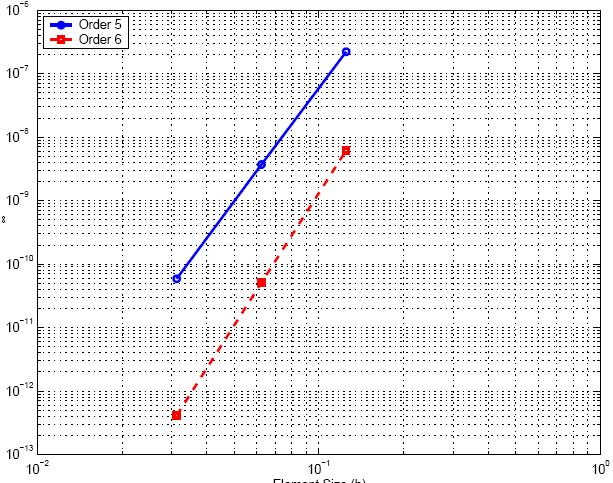
\epsfig{file = figs_dn/sinDNhconv.eps, width = 8.3cm}
    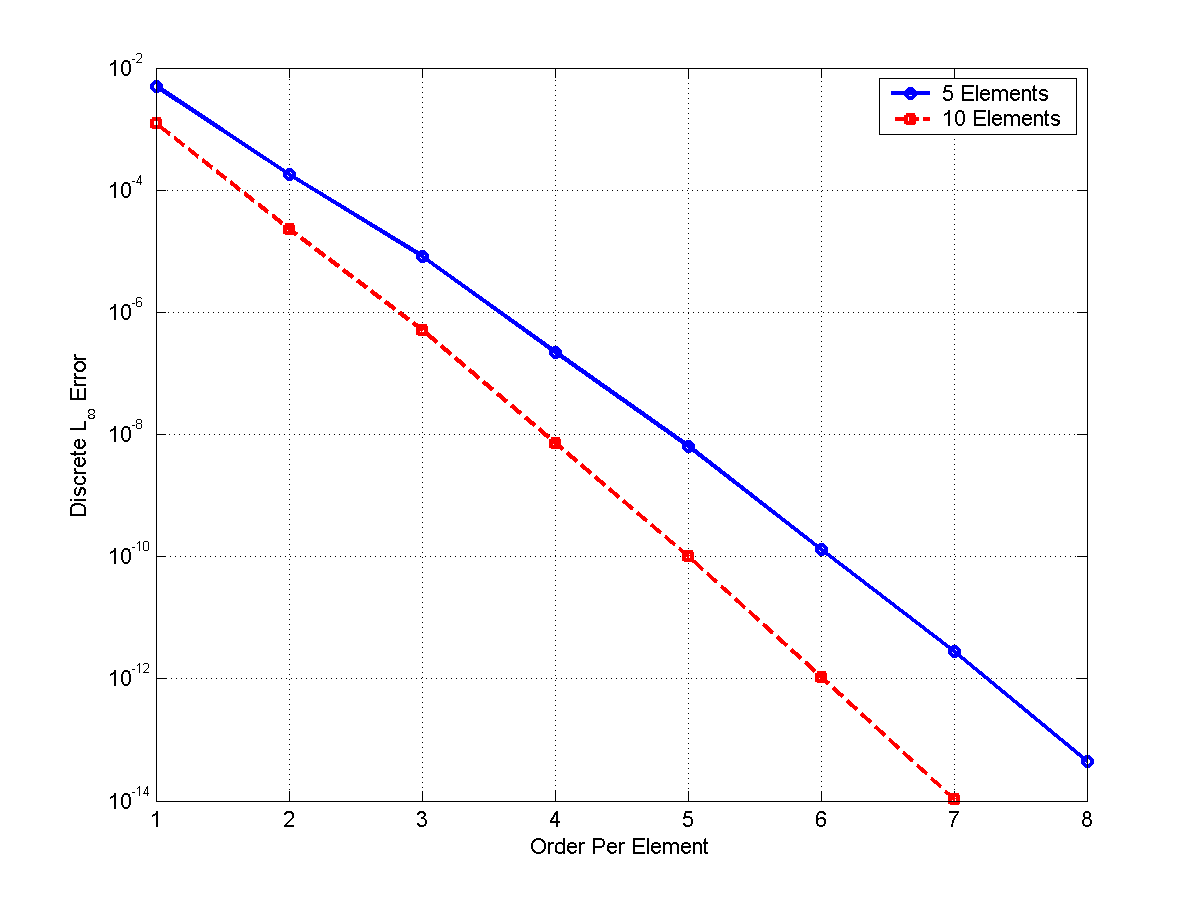
\epsfig{file = figs_dn/sinDNpconv.eps, width = 8.3cm}
    \caption{\label{sinDNconv}
(Left)Convergence with respect to discrete $L^{\infty}$ norm as a function of size of elements. This test is performed using the h-type extension with fixed polynomial order 5 and 6 respectively. Error on the Log-Log axis is demonstrating the algebraic convergence of the h-type extension.
(Right)Convergence w.r.t. $L^{\infty}$ norm as a function of size of polynomial order in semi-Log plot. It shows the exponential convergence of p-type extension for smooth solution. Two tests are performed for p-type extension with element length $0.2$ and $0.1$.
}
\end{center}
\end{figure}


\begin{table}[h]
\centering \caption{\label{hconv2t} This table shows the convergence of h-type (left) and p-type (right) resolution control done above Figure (\ref{sinDNconv}). We can see the slopes of each order $P$ is $P+1$ }
\begin{tabular}{|c|c|c|} \hline
    Polynomial order&Error($L^{\infty}$)&Slope   \\ \hline \hline
    5&$9.3603e-013$ &$5.9406$ \\ \hline
    6&$8.6542e-014$ &$6.9402$ \\ \hline
\end{tabular}
\hspace{.5in}
\begin{tabular}{|c|c|} \hline
    Element Size&Error($L^{\infty}$)\\ \hline
    0.2&$1.9385e-012$  \\ \hline
    0.1&$3.4611e-013$  \\ \hline
\end{tabular}

\end{table}

%%\{ {\it  sp1d\_ch3\_2.tex} \}

\subsubsection {High order Polynomial Solution and Its Convergence}

In this section we construct a polynomial $P_n$ of order $n$ defined on $[0,1]$, which satisfies the following.
\begin{eqnarray}
\label{pois_scrv}
    P_n(0) = 0, &P_n(1) = 1 \\
    \frac{d^k}{dx^k}P_n(0) = 0, &\frac{d^k}{dx^k}P_n(1) = 0
\end{eqnarray}
for all $k = 1, \cdots, n-2$. \\
For each $n$, we obtain polynomial $P_n$ by solving a system of
linear equations that determines the set of coefficients of $P_n$.
We use the spectral polynomial solver to approximate the second
derivative $Q_{n-2}$ of $P_n$.

\begin{figure}[h]
    \begin{center}
    \epsfig{file = Doc-Report_Fwd2D/figs_dn/ScrvH5_A.eps, width = 5cm}
    \epsfig{file = Doc-Report_Fwd2D/figs_dn/ScrvH5_N.eps, width = 5cm}
    \caption{\label{scrvsol}Example of curve that satisfies conditions (\ref{pois_scrv}) with polynomial order $n=7, 9, 12, 14, 15$. The error is $2.9239e-8$}
    \end{center}
\end{figure}

We investigate the convergences by the h-type, p-type extension of
trial functions below.

\begin{problem}
Consider the following differential equation for $u(x)$ such that
\begin{equation}
\label{poi_poly}
-r^2 \frac{\partial}{\partial r} (\sigma \frac{\partial}{\partial r}u) - r \sigma \frac{\partial}{\partial r}u - \sigma \frac{\partial^2}{\partial \theta^2}u = e^{-(r-1)^2}\{P_n(r) + (2r^2(r-1)-r)P_n'(r) - r^2 P_n''(r)\} \cos \theta,
\end{equation}
for all $r$ in $[0.1, 1.1]$ with $\sigma(r) = e^{-(r-1)^2}$.

The exact solution is known to be:
\begin{equation}
u(r, \theta) = P_n(r) \cos \theta
\end{equation}
where $r$ in $[0.1, 1.1]$ and $\theta$ in $[0, 2\pi]$.
\end{problem}

\begin{figure}[h]
\begin{center}
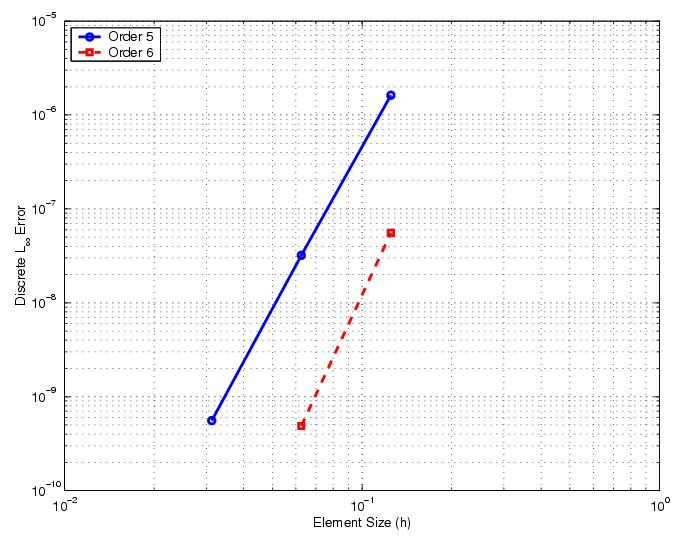
\epsfig{file = Doc-Report_Fwd2D/figs_dn/ScrvHconv.eps, width =
8.3cm} 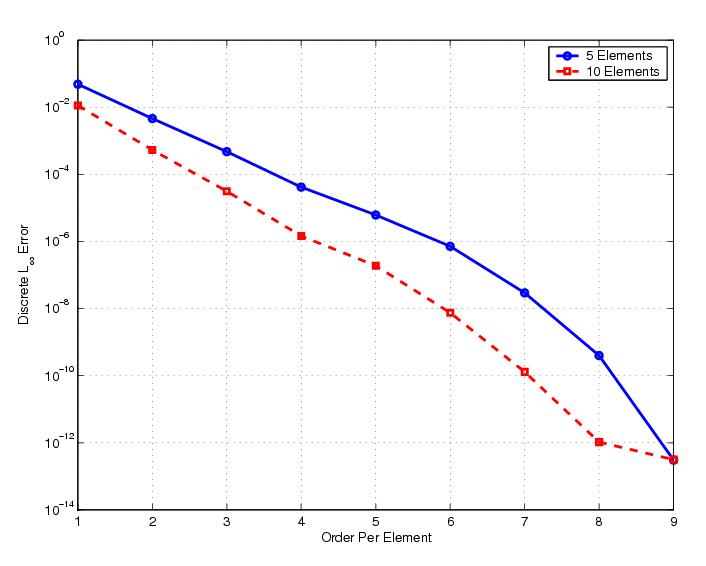
\epsfig{file = Doc-Report_Fwd2D/figs_dn/ScrvPconv.eps,
width = 8.3cm} \caption{\label{ScrvconvDN} (Left) Convergence with
respect to discrete $L^{\infty}$ norm as a function of size of
elements. This test is performed using the h-type extension with
fixed polynomials of order 3, 4, and 5 respectively. Error on the
Log-Log axis demonstrates the algebraic convergence of the h-type
extension. (Right) Convergence w.r.t. $L^{\infty}$ norm as a
function of size of polynomial order in semi-Log plot. It shows
the exponential convergence of p-type extension for smooth
solutions. The two tests are performed for p-type extension with
element lengths of $0.2$ and $0.1$. }
\end{center}
\end{figure}

\begin{table}[h]
\centering \caption{\label{hconv2t} This table shows the
convergence of h-type resolution control done above Figure
(\ref{ScrvconvDN}). We can see the slopes of each order $P$ is
$P+1$ }
\begin{tabular}{|c|c|c|} \hline
    Polynomial order&Error($L^{\infty}$)&Slope   \\ \hline \hline
    5&$8.5305e-012$ &$5.7556$ \\ \hline
    6&$4.7180e-012$ &$6.8332$ \\ \hline
\end{tabular}
\hspace{.5in}
\begin{tabular}{|c|c|} \hline
    {Element Size}&Error($L^{\infty}$) \\ \hline \hline
    0.2&$9.0616e-13$  \\ \hline
    0.1&$9.4747e-13$ \\ \hline
\end{tabular}
\end{table}

%
%\section{Conclusion}
%%\clearpage
%\{ {\it  sp1d\_ch4\_1.tex} \}

In 2-dimensional case, we looked into the theory of Spectral
Polynomial and Fourier Method and its solvability. We also
investigated the feature of convergence in the viewpoint of h/p
convergence property in comparison to classical finite element
method. By using Galerkin method, we could incorporate the weak
solution and get the problem to be changed to system of linear
equations which we can solve it by computer.

By implementing the Spectral element solver for one dimensional Poisson equation having Dirichlet and Neumann boundary conditions, we could experiment all the theory with various specific cases of high-order solutions which were hard to get acceptable convergence in a given time and resolution of domain.


%------------------------------------------------------------------------------
%   BIBLIOGRAPHY
%%\clearpage

%\{ {\it  sp1d\_chbib.tex} \}

\begin{thebibliography}{9}

\bibitem{Karniadarkis}{\bf Spectral/Hp Element Methods for Cfd},
        George Em Karniadakis, Spencer J. Sherwin, \/
        Oxford Univ Press, 1999.

\bibitem{Trefethen}{\bf Spectral Methods in MATLAB},
        Lloyd N. Trefethen, \/
        Society for Industrial and Applied Mathematics, 2001.

\bibitem{Johnson}{\bf Lecture note of Advanced Methods in Scientific
Computing},
        Christopher R. Johnson, \/
        School of Computing, University of Utah, 2002.

\bibitem{Chen}{\bf A direct spectral collocation Poisson solver in polar and cylindrical
coordinates},
        Chen HL. Su YH. and Shizgal BD., \/
        Journal of Computational Physics. 160(2), 453-469 (2000).

\bibitem{Choe}{\bf Solving One-dimensional Forward Problems using Spectral Element
Method},
        S. Choe, \/
        Project report in Computational Engineering and Science Program, University of Utah, 2004.


\end{thebibliography}



%-------------------------------------------------------------------------------
%   APPENDIX
%
%

\{ {\it  sp1d\_chapdx.tex} \}

%\clearpage
\appendix
\section {Gaussian Quadrature Formula}



\end{document}
